\documentclass[10pt,a4paper]{report}
\usepackage[utf8]{inputenc}
\usepackage{amsmath}
\usepackage{amsfonts}
\usepackage{amssymb}
\usepackage{graphicx}
\usepackage{fancyvrb}
\usepackage{float}
\DefineVerbatimEnvironment{code}{Verbatim}{fontsize=\small}
\DefineVerbatimEnvironment{example}{Verbatim}{fontsize=\small}
\author{Yapi Donatien Achou}
\title{Project 1 MEK4470}
\begin{document}

\section{question 1}

The PISO algorithm (Pressure Implicit with Splitting of Operator) is an algorithm used to find pressure and velocity in steady and unsteady flow.
It uses one predictor step and two corrector steps. Is can been seen as an extension of the SIMPLE algorithm. Consider the discretised momentum equation and the discretised continuity equation. Using a guessed pressure $p^{*}$ into the momentum equation, the velocity component ($u^{*}, v^{*}, w^{*}$) are derived. Since the pressure is guessed, the derived velocity field will not satisfy the continuity equation. To solve this problem, in a first corrector step,  a corrector pressure $p^{\prime}$ is defined as the difference between the guess pressure and the real pressure. Using the continuity equation a pressure correction equation is derived in terms of the pressure $p^{**}$. Introducing this pressure into the discretised momentum equation a velocity field ($u^{**}, v^{**}, w^{**}$) satisfying the discretised continuity equation is computed. In the second corrector step a corrected pressure $p^{***}$ is introduce in the discretised momentum equation to derive a twice corrected velocity field ($u^{***}, v^{***}, w^{***}$).\\
\\
The PISO algorithm implementation in openFoam:

1)define equation for U
\begin{code}

 fvVectorMatrix UEqn
 (
   	fvm::ddt(U)
      + fvm::div(phi, U)
      - fvm::laplacian(nu, U)
 );
\end{code}

2)solve the momentum predictor:
\begin{code}
solve (UEqn == -fvc::grad(p));
\end{code}

3)Calculate $a_{p}$ coefficient and calculate $U$
\begin{code}
volScalarField rUA = 1.0/UEqn().A();
 U = rUA*UEqn().H();
\end{code}

4)Calculate the flux
\begin{code}
phi = (fvc::interpolate(U) & mesh.Sf()) 
       + fvc::ddtPhiCorr(rUA, U, phi);
 adjustPhi(phi, U, p);
\end{code}

5)Solve the pressure equation

\begin{code}
fvScalarMatrix pEqn
 (
    fvm::laplacian(rUA, p) == fvc::div(phi)
 );
 pEqn.setReference(pRefCell, pRefValue);
 pEqn.solve();
\end{code}

6)Correct the flux

\begin{code}
if (nonOrth == nNonOrthCorr)
 {
    phi -= pEqn.flux();
 }
\end{code}

7) Correct the flux
\begin{code}

 if (nonOrth == nNonOrthCorr)
 {
    phi -= pEqn.flux();
 }
\end{code}

8)calculate continuity error
\begin{code}
# include "continuityErrs.H"
\end{code}

9)Perform the momentum corrector step
\begin{code}
U -= rUA*fvc::grad(p);
 U.correctBoundaryConditions();
\end{code}

10)repeat from 3) for the prescribed number of PISO corrector step.\\


\section{question 2}
consider the domain given by 

\begin{figure}[H]
  \caption{Computation domain} 
  \centering
    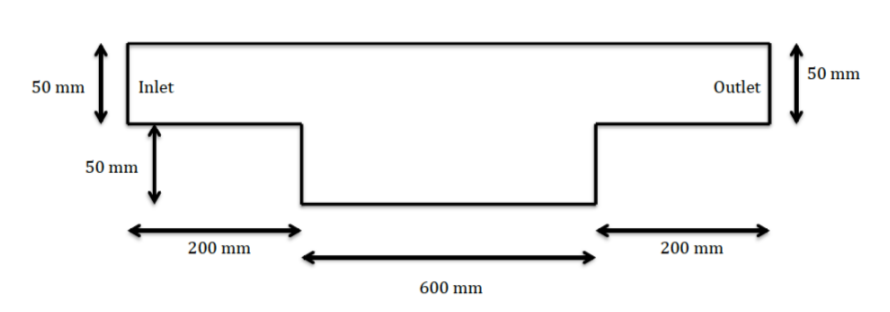
\includegraphics[width=1\textwidth]{domain.png}
\end{figure}

We want to solve this flow using the pisoFoam solver for LES model. The governing equations are given by the LES continuity equation and the LES momentum equations:

\begin{equation}
\frac{\partial\rho}{\partial t}+ div{(\rho\bar{\textbf{u}})}= 0
\end{equation}


\begin{equation}
\frac{\partial(\rho\bar{u})}{\partial t} +div(\rho\bar{u}\bar{\textbf{u}})=
-\frac{\partial \bar{p}}{\partial x}+\mu div(grad(\bar{u}))-(div(\rho\overline{u\textbf{u}}-div(\rho \bar{u}\bar{\textbf{u}}))
\end{equation}

\begin{equation}
\frac{\partial(\rho\bar{v})}{\partial t} +div(\rho\bar{v}\bar{\textbf{u}})=
-\frac{\partial \bar{p}}{\partial y}+\mu div(grad(\bar{v}))-(div(\rho\overline{v\textbf{u}}-div(\rho \bar{v}\bar{\textbf{u}}))
\end{equation}
where $\bar{u}, \bar{v}$ are the mean velocities in the $x$ and $y$ direction. $\rho$ is the density of the fluid. $\mu$ is the viscosity and $\bar{p}$ is the average pressure.\\
Boundary condition at the inlet:\\
$(\bar{u},\bar{v}) = (10 m/s, 0)$ \\
$\bar{p}=0$\\
Boundary condition at the outlet\\
$\bar{p}= 0$\\


 In figure 2 and 3 the average or mean velocity and pressure are given :

\begin{figure}[H]
  \caption{average pressure}
  \centering
    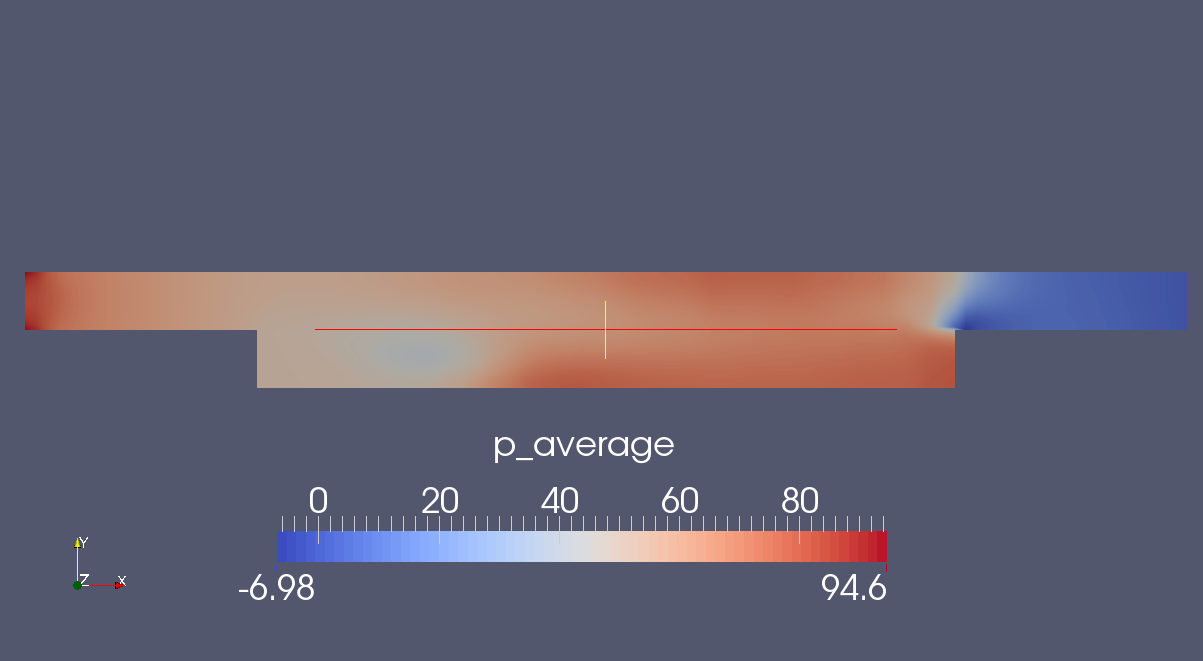
\includegraphics[width=1\textwidth]{average_P_pisofoam.png}
\end{figure}

\begin{figure}[H]
  \caption{average velocity}
  \centering
    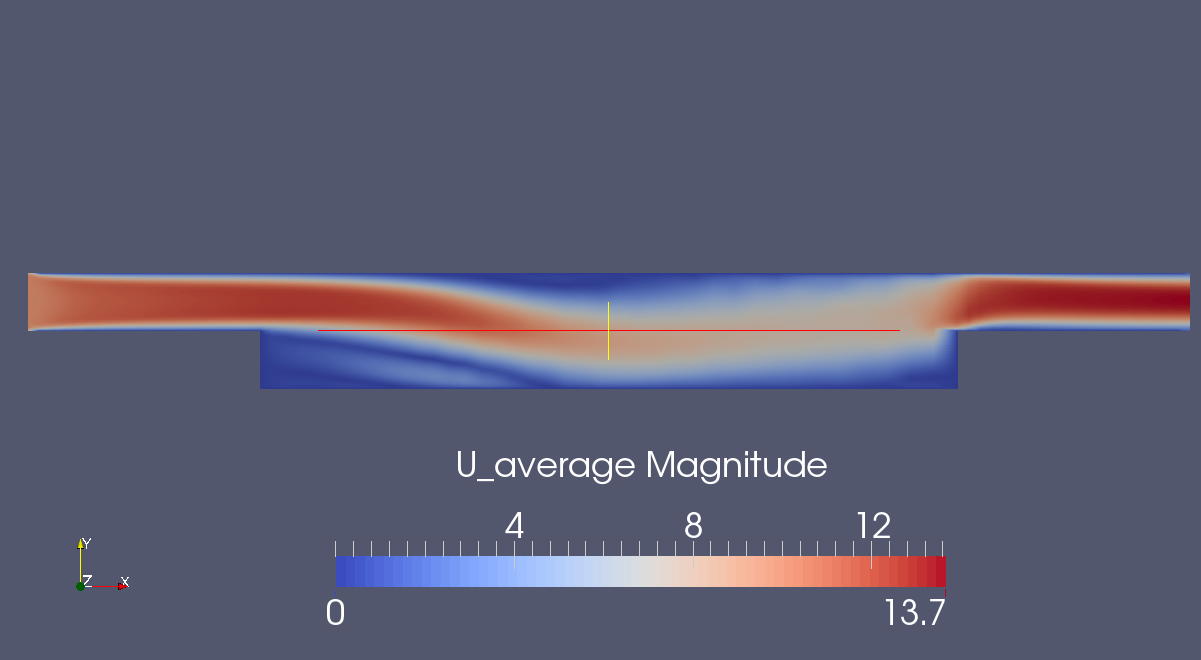
\includegraphics[width=1\textwidth]{average_U_pisoFoam.png}
\end{figure}

The size of the mesh will drive the quality of the solution.
The convection term is discretised by
the Gauss scheme (second order Gaussian integration) with a second order linear interpolation scheme (central differencing scheme). The central differencing scheme is conservative, bounded and second order accurate for Peclet number less than 2. Even though it does not posses transportiveness it requires less computational time per time step
\section{question 3}
We use pimplefoam to solve the same flow. The $k$-$\epsilon$ model equations:

\begin{equation}\label{k}
\frac{\partial(\rho k)}{\partial t}+ \nabla\cdot (\rho k\vec{U}) = \nabla\cdot(\frac{\mu_{t}}{\sigma_{k}}\nabla k) + 2\mu_{t}S_{ij}.S_{ij}-\rho\epsilon
\end{equation}

\begin{equation}\label{e}
\frac{\partial(\rho \epsilon)}{\partial t}+ \nabla\cdot (\rho \epsilon\vec{U}) = \nabla\cdot(\frac{\mu_{t}}{\sigma_{\epsilon}}\nabla \epsilon) + C_{1\epsilon}\frac{\epsilon}{k}2\mu_{t}S_{ij}.S_{ij}-C_{2\epsilon}\rho\frac{\epsilon^{2}}{k}
\end{equation}

with the eddy viscosity defined by
\begin{equation}
\mu_{t} = \rho C_{\mu}\frac{k^{2}}{\epsilon}
\end{equation}

In equation (\ref{k}, \ref{e}) $k$ is the turbulent kinetic energy and $\epsilon$ is the rate of  viscous dissipation. $ \rho$ is the density.
$c_{1\epsilon}= 1.44$, $c_{2\epsilon}= 1.92$,$C_{\mu}= 0.09$ and $ S_{ij}$ is the rate of deformation.
the boundary condition for the turbulent model are:\\
at the inlet we have:
\begin{equation}
k = \frac{2}{3}(U_{ref}T_{i})^{2} \nonumber
\end{equation}

\begin{equation}
\epsilon = C_{\mu}^{3/4}\frac{k^{3/2}}{0.07L}\nonumber
\end{equation}

where $L$ is a characteristic length and $T_{i}$ is the turbulent intensity. The initial kinetic energy is set to $k= 0.375 m^{2}/s^{2}$ and the initial dissipation energy rate to $\epsilon = 10.781 m^{2}/s^{3}$ at the inlet.
In figure 4 the average velocity is given. The convective term is discretised by using an upwing scheme satisfying transportiveness , boundness, conservativeness and is first order accurate. 
\begin{figure}[H]
  \caption{average velocity}
  \centering
    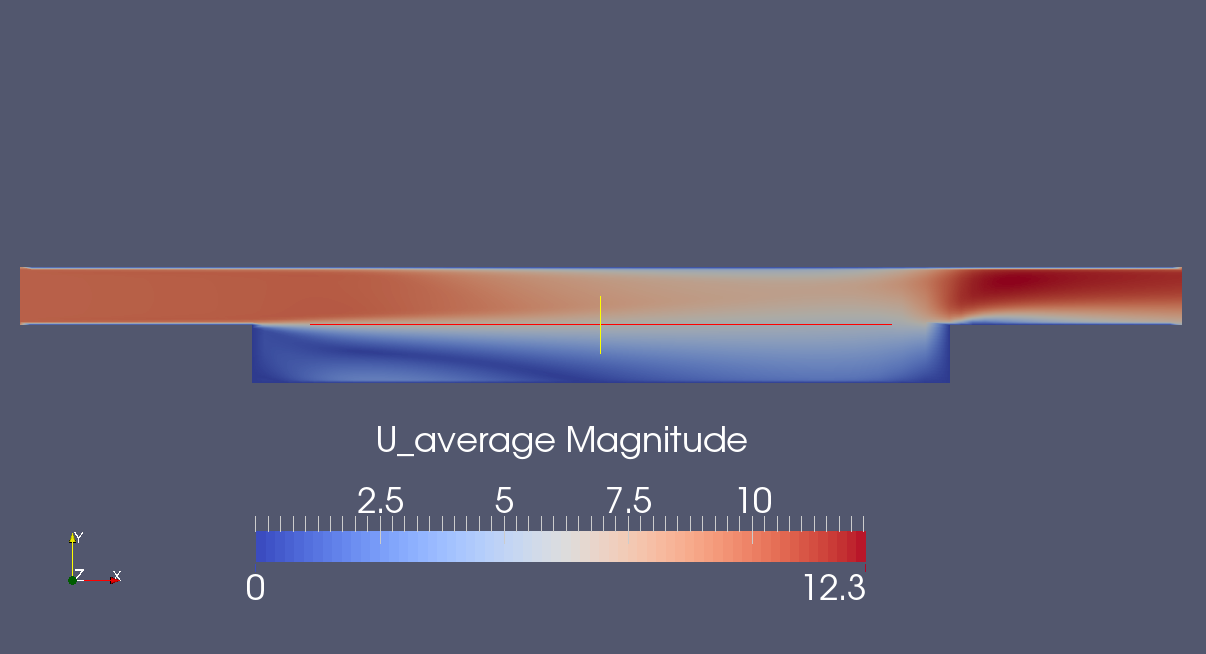
\includegraphics[width=1\textwidth]{U_average_pimpleFoam.png}
\end{figure}


\section{question 4}
pimplefoam uses large time step. It is more suitable for RANS because RANS can use coarser mesh than LES which uses more finer mesh. In RANS you use larger time step then in LES.

\section{Comparison  of result from RANS and LESS}
Figure 4 shows the magnitude of the average velocity from PimpleFoam solver using RANS. The velocity field reach steady state faster than the velocity field obtain from PisoFoam using LES from figure 2 and 3. The LES model shows more turbulence than the RANS model because there is no dissipation to dump the kinetic energy. (see video). In LES the recirculation bubbles are far from the inlet some where in the middle of the domain. In RANS the recirculation bubbles are closer to the backward step and dies out quickly as the flow reaches steady state. In the LES model there is no dissipation to dump the kinetic energy while in the RANS model the rate of dissipation $\epsilon$ is much larger than the energy used to create turbulence. As the flow progress in the RANS model, the kinetic energy used to maintain turbulence will dissipate very fast and the flow will reach steady state faster. 
\section{ question 6}
LES is not usually used as a two D model because turbulence is a 3D phenomenon.
\end{document}